% Created by Jim Finnis
% Date Wed Feb 24 13:48:57 2021

\begin{todoblock}
\begin{itemize}
\item Change getInput and getOutput docs
\item update conntypes doc
\item add Datum details
\end{itemize}

\end{todoblock}


\section{The data model}
The ``root'' of the data model is the \texttt{Document} object.
This contains:
\begin{itemize}
\item the ``main graph'' --- that is, the graph of nodes not contained
inside macros;
\item a dictionary of macro type objects (\texttt{XFormMacro}) by name,
which are local to this document --- each macro also contains a ``prototype
graph'' (see Sec.~\ref{macros});
\item the input manager and the state of the various input methods
contained in each input (see Sec.~\ref{inputs});
\item document-wide settings.
\end{itemize}
The most important parts of the model are the graph
and the data which it manipulates --- this is largely
image cube data passed between the graph nodes.
Other forms of data do exist,
but these are much simpler.

\subsection{Graph and nodes}
Graphs are directed acyclic graphs of nodes represented by the 
\texttt{XFormGraph} class. Each node is an instance of \texttt{XForm}
(short for ``transform node''). The function of each node is
determined by its \texttt{type} field, which references an
\texttt{XFormType} singleton. See Fig.~\ref{xform.pdf} for an overview,
which also shows an outline of how the main graph and macro prototype
graphs fit into the document.

\begin{figure}[ht]
\center
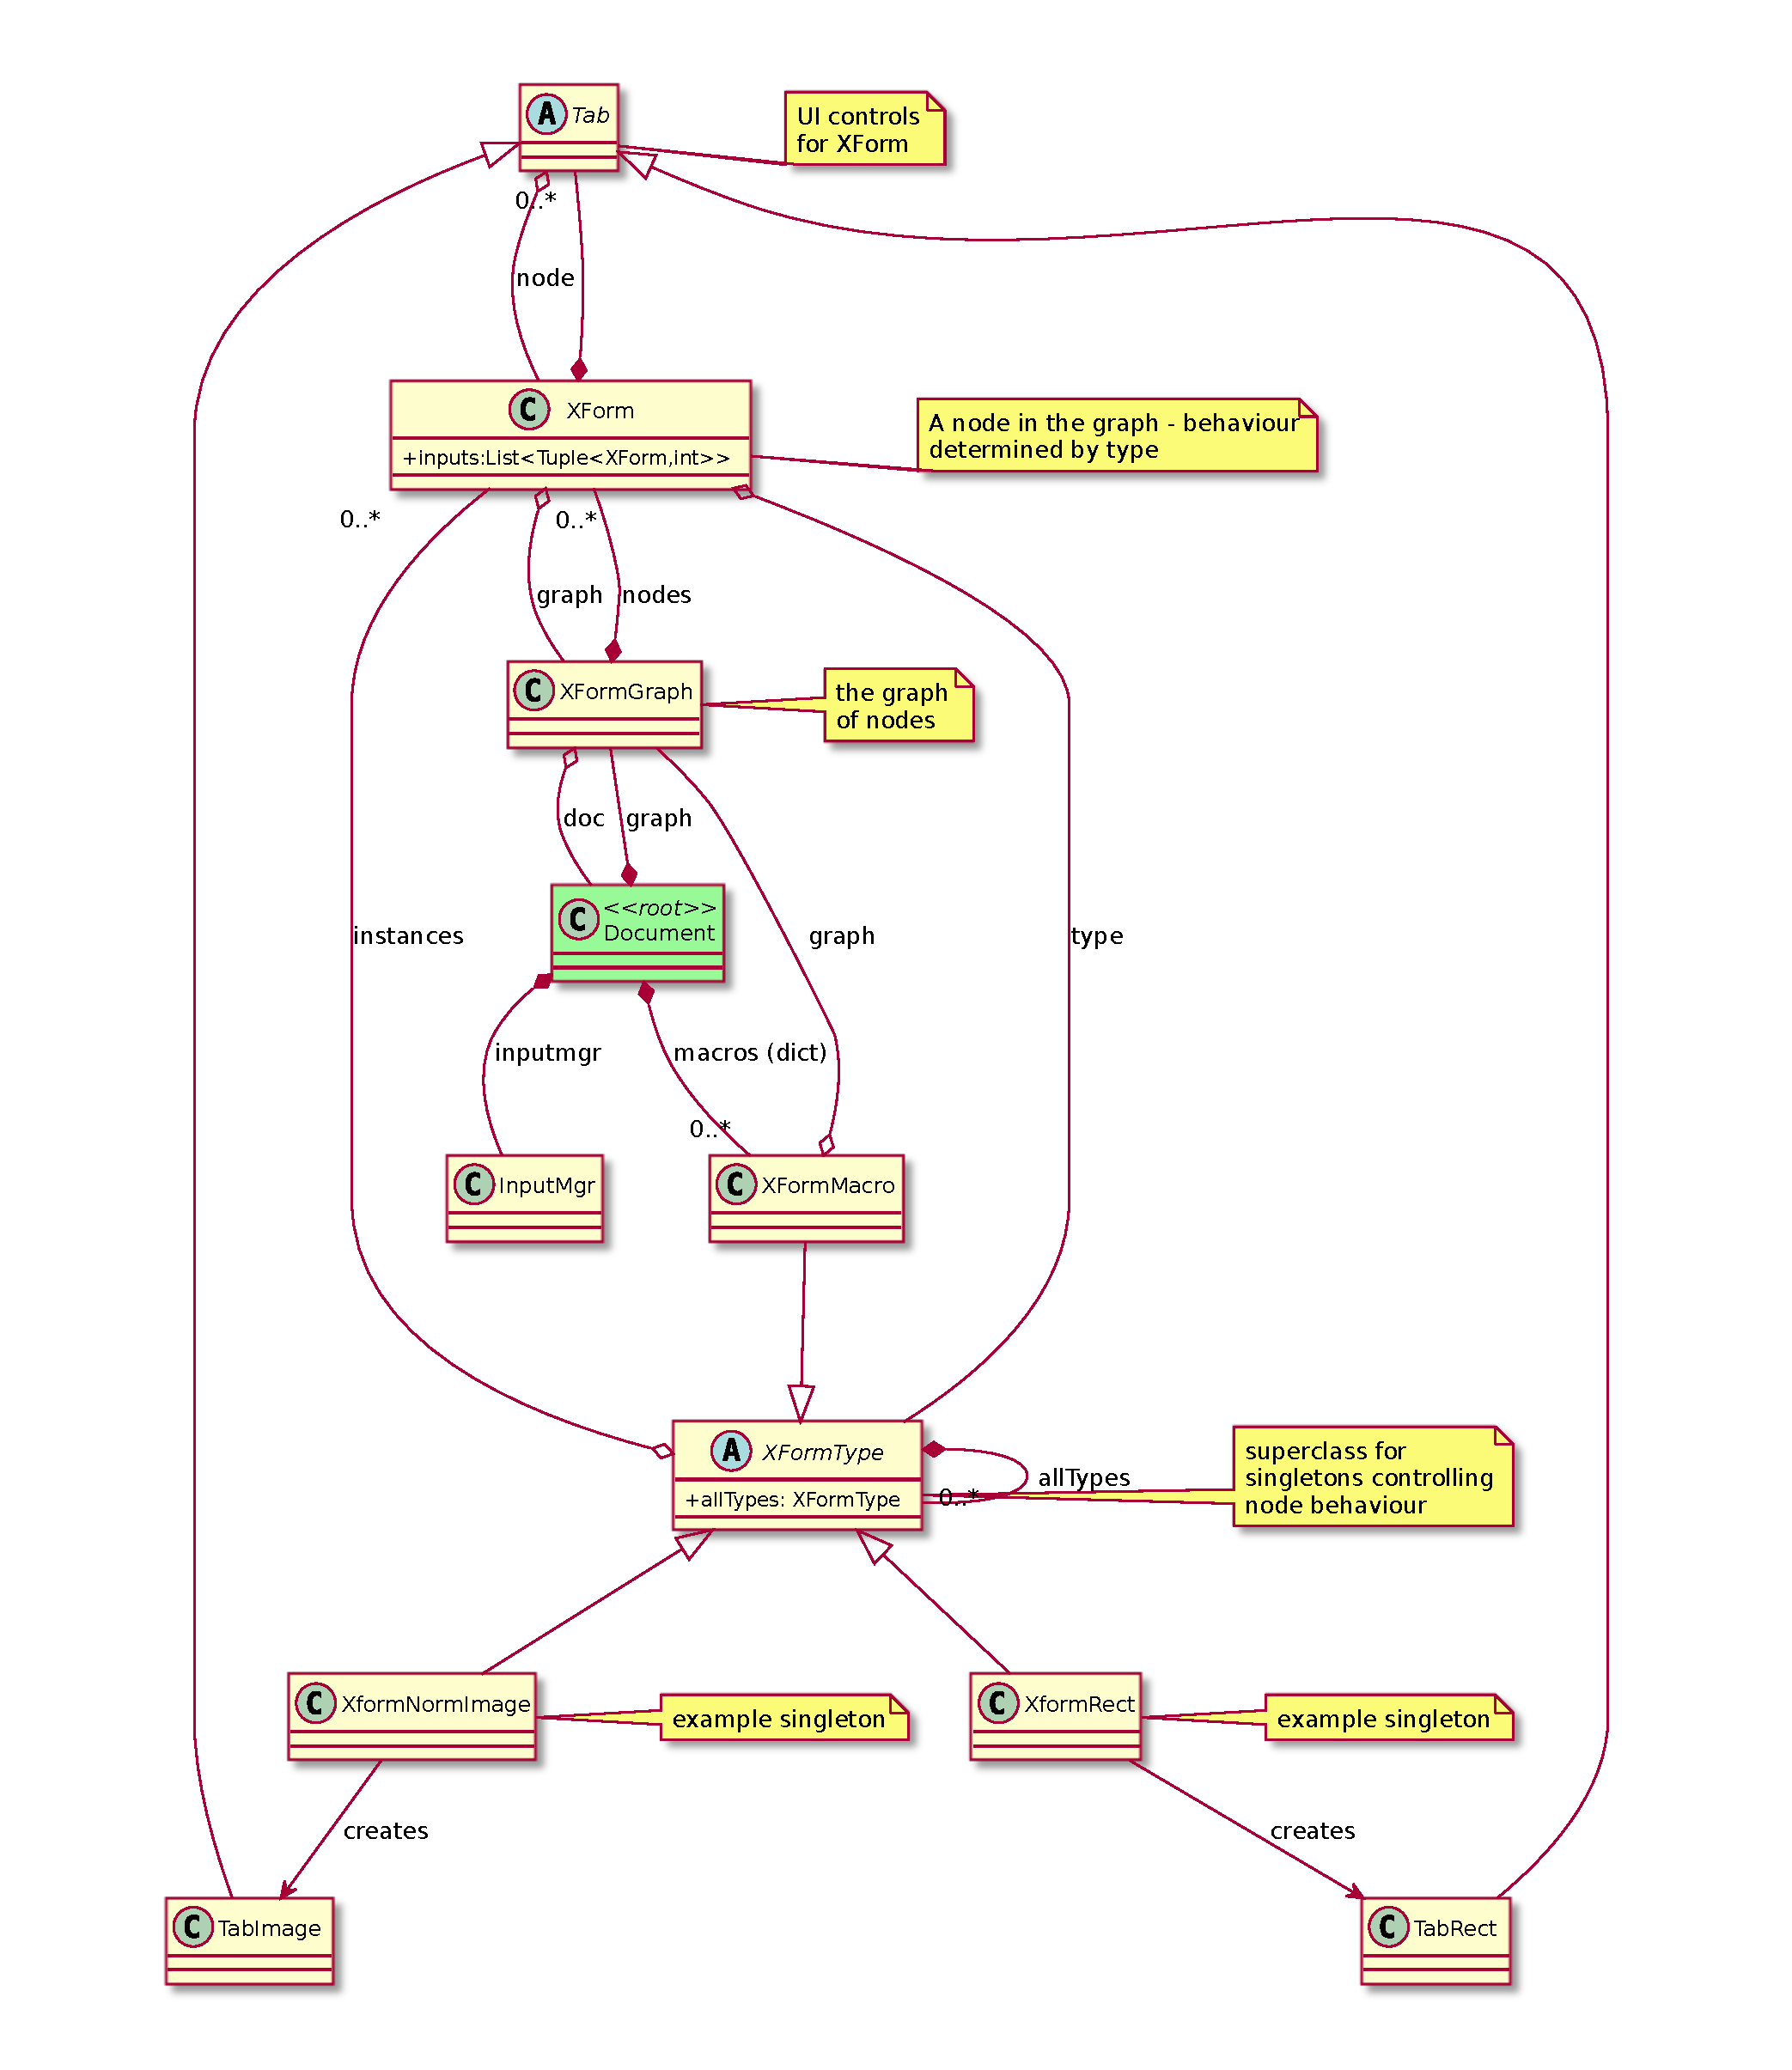
\includegraphics[width=6in]{xform.pdf}
\caption{\texttt{XForm} and graph model}
\label{xform.pdf}
\end{figure}

\subsubsection{XFormType and type registration}
\label{xformtype}
Each node type is represented by a subclass of \texttt{XFormType},
and each subclass has a singleton to which nodes of that type link.
For example, the \emph{rect} node's behaviour is specified by
the \texttt{XformRect} class, which has a singleton instance. All
\texttt{XForm} nodes which are \emph{rect} nodes have a \texttt{type} field
pointing to this singleton.

Most singletons are automatically created and registered when the class
is defined, through the \texttt{@xformtype} decorator and \texttt{createXFormTypeInstances()}. 
The decorator stores the required information ---- name, class, constructor arguments etc. ---
into a list, while \texttt{createXFormTypeInstances()}, which runs just before the app starts (as
late as possible) does the following for each entry:
\begin{itemize}
\item Creates an instance of the class;
\item Creates an MD5 hash of the class' source code which is stored
inside the type singleton for version control;
\item Changes the semantics of the class constructor so that
it always returns the instance we just created (thus making the class
a singleton).
\end{itemize}
The reason for the deferred instantiation of the type objects is to ensure that all user
hooks are run before the instantiation (so that \emph{expr} function hooks [Sec.~\ref{writingfuncs}]
work).

The base constructor for \texttt{XFormType} adds the singleton
to a dictionary class variable \texttt{allTypes}, so we can always
obtain the singleton object and create new nodes which perform that
node type. In addition, each type singleton has a ``group'' field which 
determines where in the palette to create a construction button for the type.

Some other \texttt{XFormType} objects are dealt with differently:
\begin{itemize}
\item Macros are represented by \texttt{XFormMacro} objects --- a subclass
of \texttt{XFormType}. However, these
are stored inside the document, not in the global type
dictionary --- this ensures that macros are document-local\footnote{The
ramifications of macros being global to the application are problematic:
consider opening a file with a macro ``foo'' defined one way, and then
opening another file with a different definition of the same macro!}
\item Some nodes are registered normally in \texttt{allTypes} but are given
a ``non-existent'' group name to stop them appearing in the palette.
These include the \texttt{XFormDummy} type, assigned to nodes whose
type cannot be found; and macro connectors which can only be created inside
macros.
\end{itemize}

\subsubsection{XFormType methods}
In order to perform a node's action, the type classes must contain
the following methods:
\begin{itemize}
\item \texttt{init(node:XForm)} : initialise any extra data inside
the node required to perform this type's behaviour
\item \texttt{perform(node:XForm)} : perform this node's behaviour ---
read any inputs, manipulate the data, set the outputs.
\item \texttt{createTab(node:XForm, window:MainWindow)} : create a UI tab to edit/view this node.
\end{itemize}
Several other methods may optionally be overridden.

\subsubsection{Linkage}
\label{linkage}
\texttt{XForm} node objects are linked together by their inputs.
Each \texttt{XForm} contains an \texttt{inputs} list indexed by
input number. The length of this list is determined by the number
of inputs the type object specifies. Each entry is a $(node,output)$
tuple where $node$ is a reference to another \texttt{XForm} and
$output$ is the index of an output on that \texttt{XForm}.

Methods are provided in \texttt{XForm} for connecting and disconnecting nodes
(also checking for cycles and providing basic type checking), and getting
inputs and setting outputs inside the type's \texttt{perform()} method.

The number and types of inputs and outputs is set inside the 
constructor for the \texttt{XFormType} singleton, by using methods
to add these connectors. They are then indexed in order of creation.
For example, the \emph{inset} \texttt{XFormType} has the constructor:
\begin{lstlisting}
    def __init__(self):
        super().__init__("inset", "regions", "0.0.0")
        self.addInputConnector("img", Datum.IMG)    # input 0
        self.addInputConnector("inset", Datum.IMG)  # input 1
        self.addInputConnector("rect", Datum.RECT)  # input 2
        self.addOutputConnector("", "img")
\end{lstlisting}
The arguments for these methods are $(name,type,description)$ where the name
is often empty (it just shows a hint) and the description is optional (it appears
in help text). The type is a \texttt{datum.Type} value --- these are stored
by name as static members of \texttt{Datum}.

Within an executing graph, the data between nodes is stored as an \texttt{xform.Datum}
object containing the type and value. Inside the node type's \texttt{perform()} method,
we typically do something like:
\begin{lstlisting}
    node.setOutput(0, Datum(Datum.IMG, img))
\end{lstlisting}
which sets output 0 to hold the image (i.e.\ \texttt{ImageCube}) stored in \texttt{img}.
Fetching data from an input is also done in \texttt{perform()}, and takes two forms. The
first returns a \texttt{Datum}:
\begin{lstlisting}
    datum = node.getInput(0)
\end{lstlisting}
while the second examines the datum internally, and returns the value field if
the type matches or None if it doesn't:
\begin{lstlisting}
    image = node.getInput(0, Datum.IMG)
\end{lstlisting}
Note that None is a permissible value in \texttt{setOutput()}, which \texttt{getInput()} will
always return as None.

\subsubsection{Overriding types and the variant type}
It is possible for an individual \texttt{XForm} node to override the input and output types
set in its \texttt{XFormType}, by setting values in the \texttt{inputTypes} and \texttt{outputTypes}
array. This is used in macros and mathematical operations. Often the ``default'' type is \texttt{Datum.VARIANT},
which is a special type which must be overriden by some user action before the node becomes useful. A variant connection
shows as crosshatched, and cannot be connected until its type is changed.

\subsection{Performing the graph}
\label{graphperform}
The graph needs to be ``performed'' --- its nodes executed --- whenever
the data changes, which is generally whenever the graph is edited,
a node control changed in a tab, or an input is changed (see Sec.~\ref{inputs}
below).
This is done by calling \texttt{changed()} on the node's graph (or on the tab itself).
The \texttt{XFormGraph.changed()} method takes a node, and either calls
\texttt{performNodes()} on the main graph passing in that node, or, if the
node is inside a macro prototype graph (q.v.), copies the prototype graph to
all its instances and runs \texttt{performNodes()} for all those instances
(see Sec.~\ref{macroineff} for why this is a problem).

The \texttt{XFormGraph.performNodes(node=None)} method itself takes a single
argument and performs either the entire graph or a portion of the graph
starting at a particular node. If the argument is None, the internal list of
all nodes in the graph is traversed looking for nodes with no inputs and these
are performed. If the argument is not None that node is performed. Nodes are
performed by calling their \texttt{perform()} method. This will recursively
run the child nodes, but only when they are ``ready to run'' (all their inputs
have been set). 

\clearpage
\subsubsection{Performing a node}
The \texttt{XForm.perform()} method will run a node, and recursively run all child nodes, although
there are some complexities here (mainly to accommodate macros). It will not perform the node if it 
has already run in this call to \texttt{performNodes()} or if it is not ready to run (some inputs do not yet have values):
\begin{algorithmic}
\IF{node has not already run \textbf{and} node is ready to run}
\STATE clear all outputs
\STATE run the node type singleton's \texttt{perform()} method on the node
\STATE mark node as having run
\FORALL{$t$ in open tabs for this node}
\STATE $t$\texttt{.nodeChanged()}
\ENDFOR
\FORALL{$c$ in child nodes}
\STATE perform node $c$
\ENDFOR
\ENDIF
\end{algorithmic}
A node is ready to run if it has no inputs which do not yet have values set. This is
determined by checking the outputs of the nodes from which the inputs come to see if
they have yet been set with values. The \texttt{performNodes()} method is called from only two places:
\begin{itemize}
\item \texttt{XFormGraph.changed(node)}: when the graph or a node in a graph has been changed. This is the most
frequent call, and is typically called with a node to avoid running the whole graph. The node is passed down into
\texttt{performNodes()}).
\item \texttt{XFormMacro.perform(node)}: when a node which contains a macro instance is being performed (see
Sec.~\ref{macros} for more details).
\end{itemize}
The \texttt{XFormGraph.changed()} method is called from several places:
\begin{itemize}
\item \texttt{XFormGraph.runAll()} : called when a graph is explicitly run.
\item \texttt{XForm.disconnect()} and \texttt{XForm.connect()}: when connections between nodes are made or broken.
\item \texttt{XForm.setEnabled()}: when a node is enabled or disabled.
\item \texttt{Tab.changed()}: when a tab signals that a node it controls has had a parameter change.
\item \texttt{XFormGraph.deserialise()}: when a graph has been loaded.
\end{itemize}

\subsubsection{Error handling}
\label{errorhandling}
Error handling is generally required in three cases:
\begin{itemize}
\item connection type mismatch discovered at connect time,
\item connection type mismatch discovered at perform time,
\item other errors at perform time.
\end{itemize}
The first is dealt with using the data type system
in \texttt{datom.py}: each connection (input and output) has a string
type and the connections must match, or they will not be made. An input
of type ``any'' can accept any type. Additional checks are made to avoid
cycles.

The other types of error are both handled inside the node's \texttt{perform()},
and take two forms:
\begin{itemize}
\item either the type's \texttt{perform()} throws an \texttt{XFormException}, which
is handled by \texttt{XForm.perform},
\item or \texttt{perform()} completes but perhaps shows an empty image,
and calls \texttt{setError(exception)} to set the error state.
\end{itemize}
In both cases \texttt{setError()} will print a message to console and
set an error state in the node. This error state
will have been cleared in all nodes before the graph is performed. A redraw of the
entire graph is done after the graph is performed to
draw those nodes in an error state differently, showing the 
brief error code passed into \texttt{XFormException}. The error
will also be shown in the tab for that node and in its ``help box''
(opened by clicking the box in the corner).

\subsection{Inputs}
\label{inputs}
Inputs are components which take external data from the DAR or from files and
bring them into PCOT. They are considered part of the document, but not part
of the graph of nodes which appears in the right-hand pane. This may sound
like an odd choice, but there are good reasons for it:
\begin{itemize}
\item We can change the graph without changing the input files: this
means we can set up an input from the DAR (which may be complex) and
then load an entirely different processing graph to view it a different way.
This also permits the use of ``template'' graphs, which can be loaded
to perform a piece of standardised processing but do not change the inputs.
\item Conversely, we can change the inputs without changing the graph.
This means we don't have to play ``hunt the input node'' if we want
to process another piece of data.
\end{itemize}
Clicking on an input at the top of the window will open the the editor for
that input. This consists for some buttons, one for each input method, and a
panel for editing the current method's data. By default the method is
``null'', which means ``no input.'' Clicking on another button will change the
active input method and allow it to be edited.
To bring the data into the graph, an \emph{input} node can be created from
the palette.
How inputs work is summarised in Fig.~\ref{inputs.pdf}:
\begin{figure}[ht]
\center
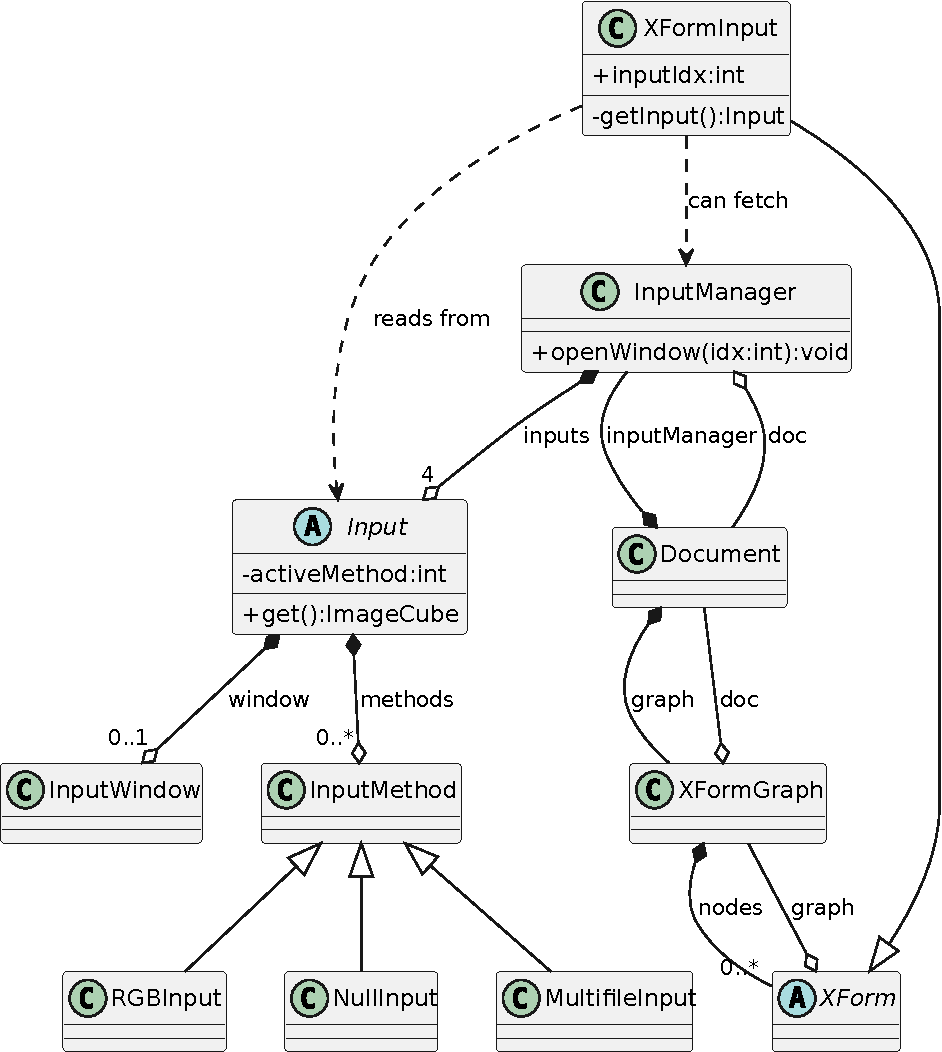
\includegraphics[width=5in]{inputs.pdf}
\caption{Input system}
\label{inputs.pdf}
\end{figure}
\begin{itemize}
\item Documents own an \texttt{InputManager}.
\item The \texttt{InputManager} owns one \texttt{Input} object for each input.
\item Each \texttt{Input} has a number of input method objects,
each of which is of a different subclass of \texttt{InputMethod}.
These handle different kinds of input: RGB file, multifile, null (does nothing)
and eventually different kinds of DAR input. Although all these methods are
always present (for persistence reasons), only one is active. An index
to the active method is stored in \texttt{Input}.
\item the \texttt{Input} may also have an \texttt{InputWindow}, if its
UI window is open. This will contain a set of widgets, each of which is
subclass of \texttt{MethodWidget}, one for each input method. Only the widget
corresponding to the active method will be visible.
\end{itemize}
Code for the inputs is the \texttt{pcot.inputs} package, except for the UI
code which is in the \texttt{pcot.ui.inputs} module.

\clearpage
\subsection{Image data}
Most classes making up the image data model are declared in the
\texttt{pancamimage.py} file, including the main \texttt{ImageCube} class.
Some additional classes describing where images can come from are in
\texttt{channelsource.py}. The model is shown in outline in
Fig.~\ref{image.pdf} although some links to channel sources and mapping from
nodes are omitted; these will be explained later.

\begin{figure}[ht]
\center
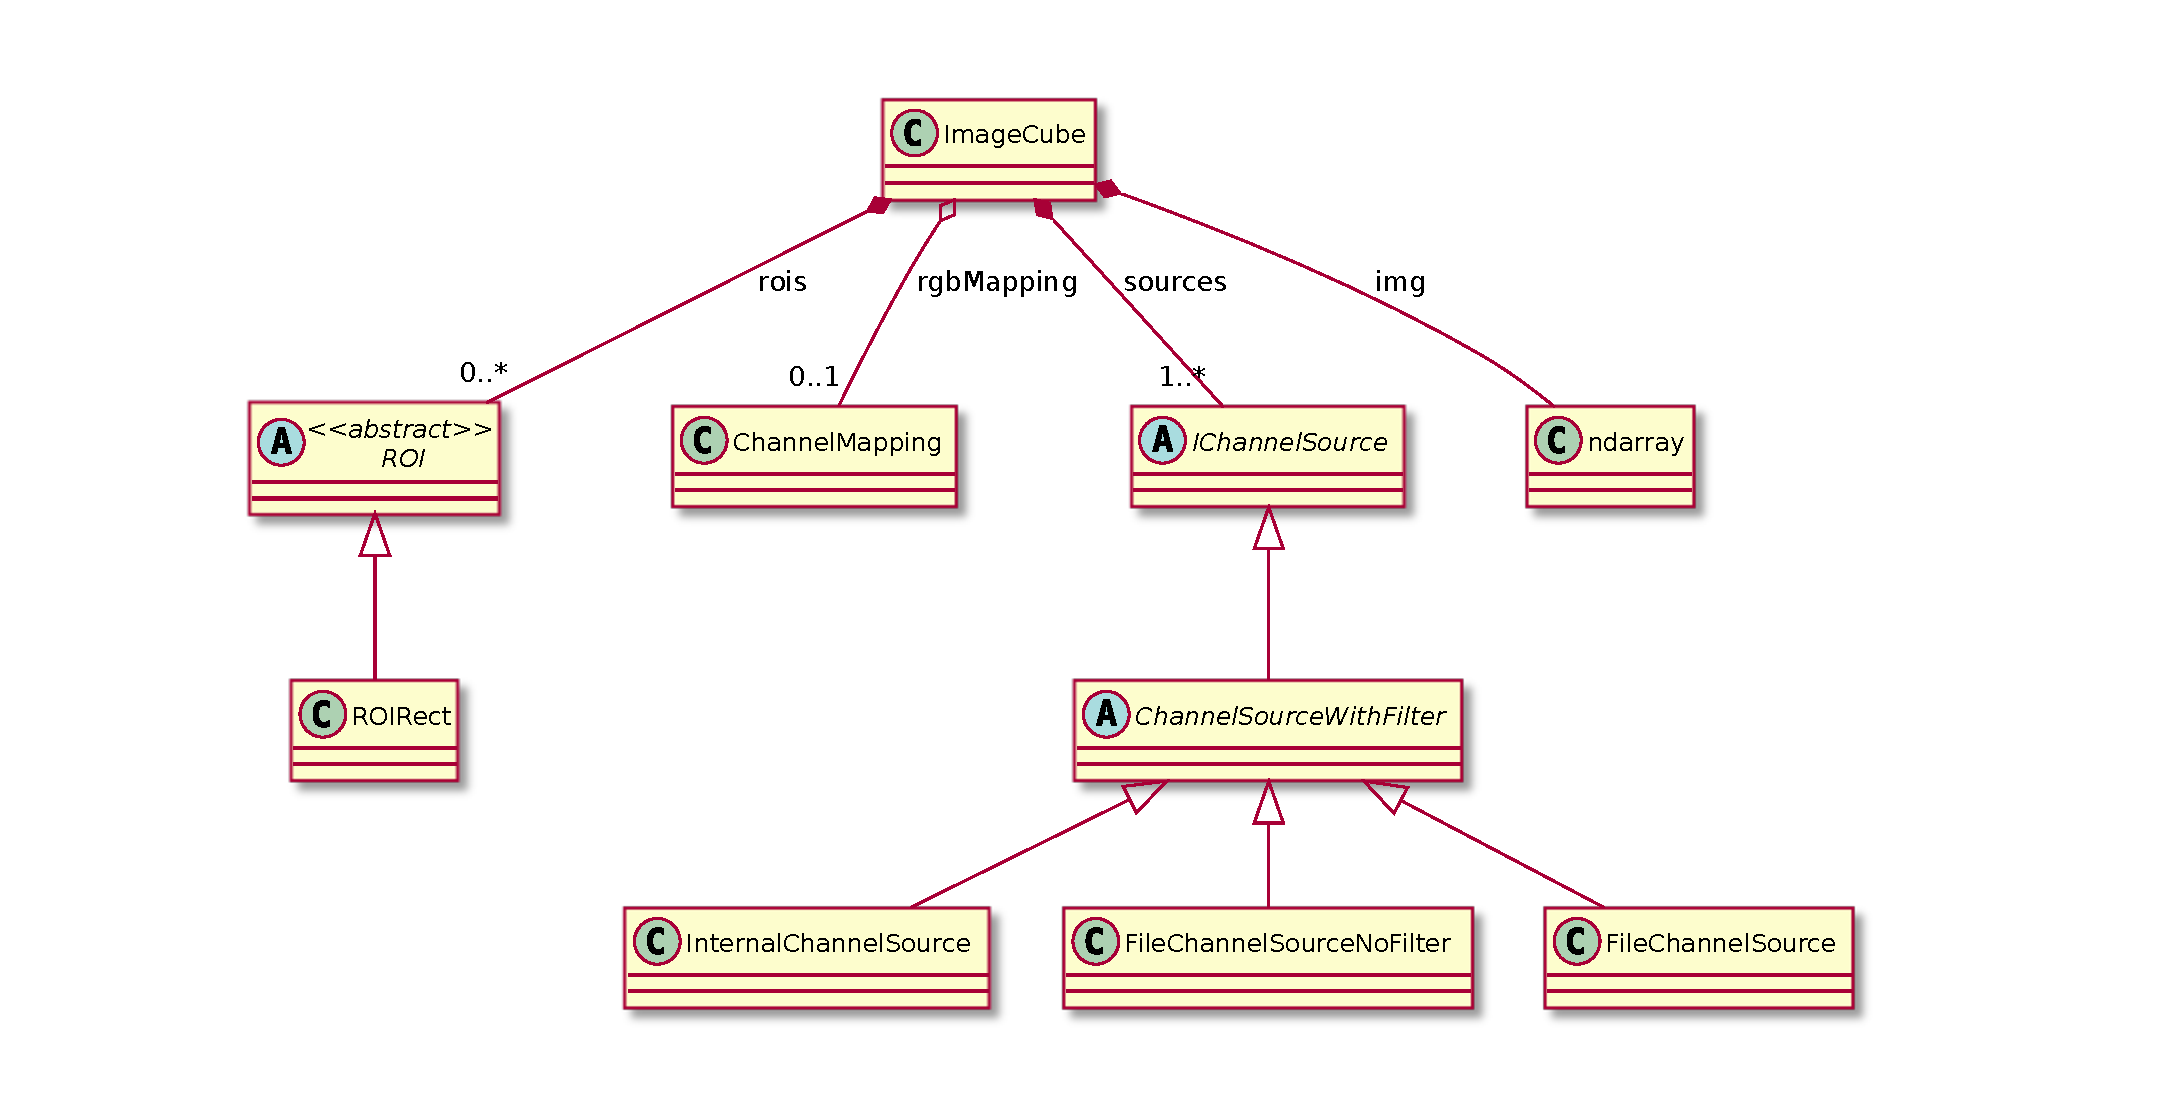
\includegraphics[width=7in]{image.pdf}
\caption{Outline UML class diagram of image model}
\label{image.pdf}
\end{figure}

The main class is \texttt{ImageCube}: this encapsulates a numpy array
\texttt{img}
which is the actual image data cube. This is either a 
$w \times h \times depth$ array for genuine cubes with multiple channels,
or a $w \times h$ array for a single channel image. The data type is 32-bit floating
point, and images are typically normalized to the range [0,1].

\begin{notebox}
In this document I have a tendency to refer to image data as both ``image'' and ``image cube.''
Both terms refer to the same thing: an array of floating point image data, with 1 or more channels (slices)
of information. There is no upper limit on the number of channels in an image (or image cube)
beyond system memory.
\end{notebox}


\subsubsection{IChannelSource and its implementations}
Each \texttt{ImageCube} has a number of channels, and for each channel there must be a corresponding
entry in its \texttt{sources} list. This describes where that channel came from, so that (typically) filter
information can be preserved, where appropriate, through the graph. The sources for each channel are a set
of \texttt{IChannelSource} objects. For example, if an image was loaded through the RGB loader, it might
have three ``fake'' channel sources for red, green and blue. Thus the sources will be 
\begin{v}
[ {RED}, {GREEN}, {BLUE} ]
\end{v}
i.e.\ a list of three sets, each with a single source.
If the image is then converted to greyscale, this could
become
\begin{v}
[ {RED,GREEN,BLUE}, {RED,GREEN,BLUE}, {RED,GREEN,BLUE} ]
\end{v}
because each channel now contains information from the red, green and blue channels in the source file.
The \texttt{RED}, \texttt{GREEN} and \texttt{BLUE} values refer in this case to \texttt{FileChannelSourceNoFilter} objects
which contain ``fake'' filter information and a filename identifier.
Each \texttt{IChannelSource} contains methods for accessing:
\begin{itemize}
\item an \textbf{identifier string} for the source from which the channel was acquired (typically a filename or data ID);
\item a \textbf{filter} and methods for obtaining the filter name, filter position and an actual filter reference (for extra data such as centre wavelength) (note
that much of this information will be ``fake'' for images loaded from plain RGB files);
\item methods for getting string descriptors for this source.
\end{itemize}

Nodes generate and process this information in different ways. For example, a
\emph{gradient} node takes a single channel and converts it into an RGB image
with a colour gradient: here, the output image's sources are ``internal RGB''
sources with no identifier or sensible filter data because the output's colour
is entirely artificial. In contrast, a the \emph{curve} for performing a
sigmoid function on all channels of an image will give the output image the
same sources as the input image.

Sources are used to keep track of each channel as it moves through the graph
so they can be processed and displayed appropriately: Fig.~\ref{app.png} shows
a typical node in the ``node controls and output'' section. This section, as
it does in many nodes, contains a ``canvas'' displaying an image. Above the
canvas are three combo boxes which select the channels in the image cube to
display on the canvas, and these are typically labelled by a string generated
from the source data for each channel (along with the index). Sources are also
used to select channels to combine and manipulate in those nodes which do so.

\subsubsection{RGB channel mappings}
The previous section briefly mentions the three RGB mapping combo boxes at the
top of the canvas component in the node controls in Fig~\ref{app.png}. In
canvases --- components which display images --- a multi-channel image cube
must be displayed as RGB data. The combo boxes control how this is done, and
the data is made persistent in a slightly complicated way, as shown in Fig.~\ref{rgb.pdf}.

\begin{figure}[ht]
\center
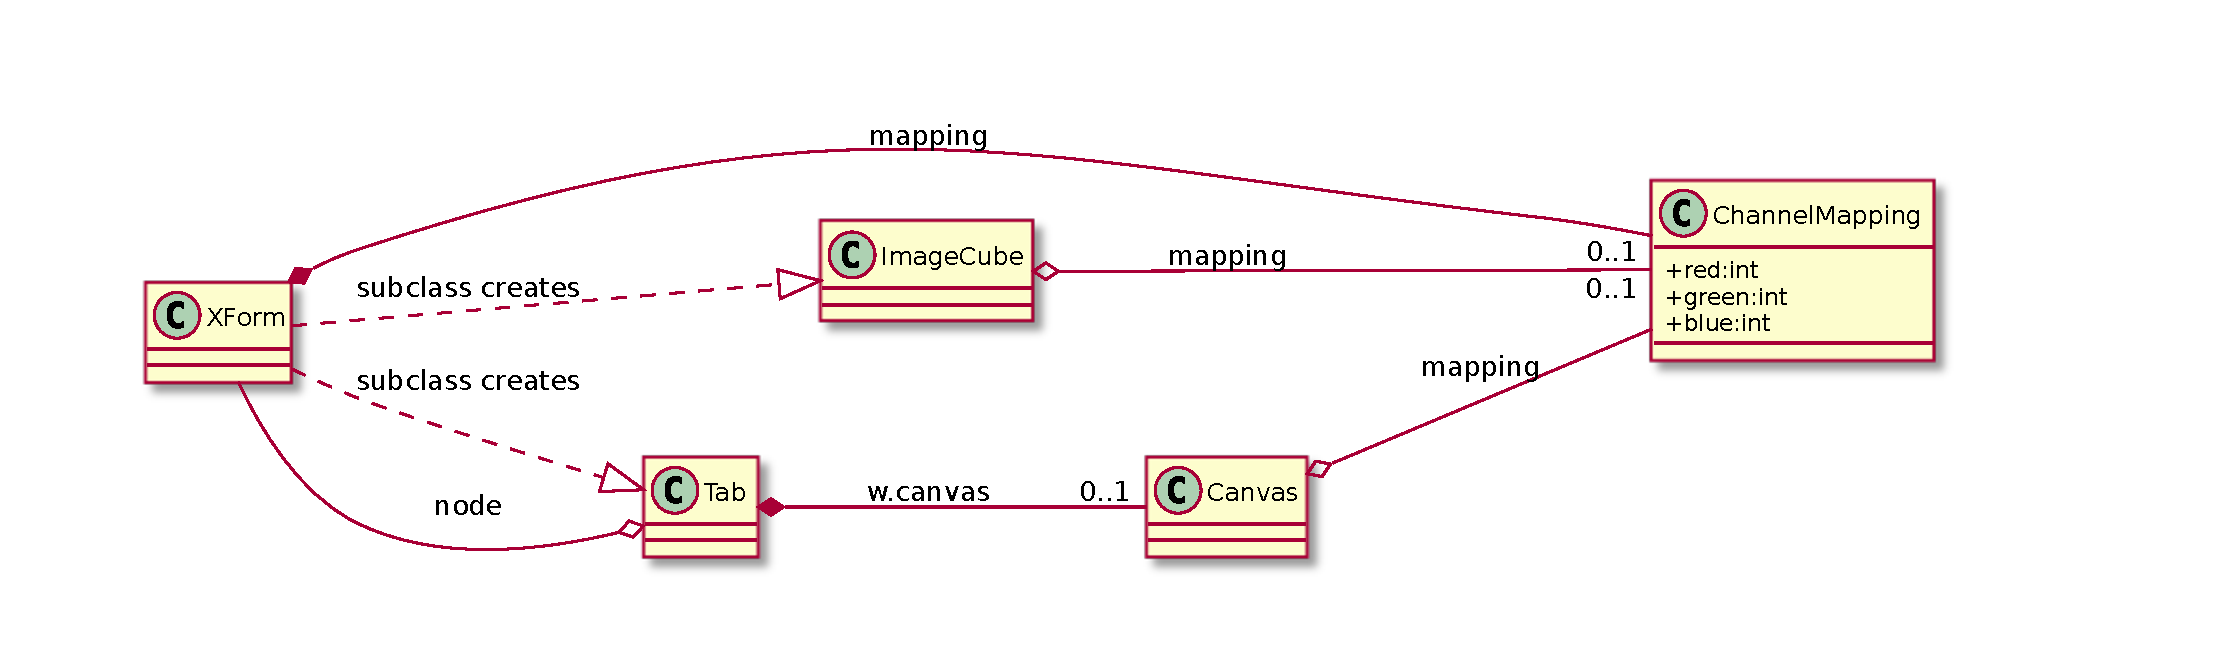
\includegraphics[width=6in]{rgb.pdf}
\caption{RGB mapping classes}
\label{rgb.pdf}
\end{figure}

The relationships will hopefully become clearer when I come to describe how nodes work in more
detail, but for now:
\begin{itemize}
\item A \texttt{ChannelMapping} object consists of three integers giving the indices of 
the channels in an image cube to display in the red, green and blue channels on screen.
\item An \texttt{XForm} (i.e.\ a node) may need to show an image on a canvas. If so, it 
will use the \texttt{mapping} field in \texttt{XForm} to store a mapping. This is provided
as a convenience, not all node classes will use it. Some may need to create more if they 
display more than one image.
\item When an \texttt{XForm} creates an image for display or passes
one through, it sets the mapping of the image to the mapping of the node. This is used in the
\texttt{rgb()} method to generate the RGB representation.
\item When an \texttt{XForm} is opened for modification, it creates a subclass of \texttt{Tab}.
This will contain a \texttt{Canvas}, which is given a reference to the mapping inside the
\texttt{XForm}. It needs this so that the mapping can be modified even when no image is present.
\end{itemize}
This may seem rather redundant, but
\begin{itemize}
\item The mapping must be be owned by the node, so it can be serialised and persists when
there is no image and no open tab.
\item We must have a reference to the mapping in the canvas, so it can be manipulated by
the combo boxes even when no image is present.
\item Finally, we need a reference to the mapping in the image so that \texttt{rgb()} can be called
on the image when it is input into another node. This is used in nodes like \emph{inset}, which
operate entirely on RGB representations --- it's much neater if these are the RGB representations
output by the nodes which feed in.
\end{itemize}
A few nodes have an extra complication --- they may output an RGB representation. In this case, the RGB conversion
needs to be done inside the node itself for output, rather than inside the canvas solely for display. A good node
to study for details on how to do this is \emph{rect}. In essence, the Canvas is told to display the ``premapped''
RGB image generated inside the node's \texttt{perform()} method. It is also given a node reference so that
the node can be performed again (thus regenerating the RGB image) whenever a mapping combo box is changed.

\subsubsection{Regions of interest}
Regions of interest belong to images, and modify how nodes process those
images. They are added to images by region of interest nodes such as
\emph{rect}. Figs.~\ref{app.png} and \ref{graph.png} show this in action:
\begin{itemize}
\item A file is read in, producing an image cube
\item A \emph{rect} node adds a region of interest to this image. The outputs are:
\begin{itemize}
\item the image with the rectangle added to its list of ROIs;
\item the image cropped to the bounding box of the list of ROIs (at the moment, just this rectangle)'
\item an RGB representation of the image (according to the previous node's canvas RGB mapping);
annotated with the rectangle and some text, and also an ROI added describing the rectangle;
\item the rectangle datum itself.
\end{itemize}
\item a \emph{decorr stretch} takes the annotated RGB representation output and imposes a decorrelation
stretch --- but only on the regions of interest in the image (in this case, inside the rectangle)
\item a \emph{histequal} node performs a histogram equalisation, again honouring the regions of interest
which have been passed through the previous node unchanged.
\end{itemize}
As shown in Fig.~\ref{image.pdf}, each image contains a list of \texttt{ROI} objects,
each of which is an instantiation of a subclass of \texttt{ROI}. 

To honouring regions of interest inside a node's \texttt{perform()} method:
\begin{itemize}
\item \texttt{ImageCube.subimage()} will return a \texttt{SubImageCubeROI} object. This encapsulates
a numpy array containing the image bounded to a rectangle around the regions of interest and
a boolean mask (again as a numpy array) specifying which pixels in this rectangle are actually
in regions of interest.
\item The manipulation can now be performed on the \texttt{img} field of this ``subimage,'' but
only on those pixels whose values are true in the corresponding \texttt{mask} field.
\item The modified pixels can be ``spliced'' into the original image cube, creating a new image
cube, using the \texttt{modifyWithSub} method.
\end{itemize}
This example shows the operation of the decorrelation stretch:
\begin{lstlisting}[language=Python]
    def perform(self,node):
        img = node.getInput(0, Datum.IMG)
        if img is None:
            node.img = None
        elif not node.enabled:
            node.img = img
        elif img.channels != 3:
            ui.error("Can't decorr stretch images with other than 3 channels")
        else:
            subimage = img.subimage()
            newimg = decorrstretch(subimage.img, subimage.mask)
            node.img = img.modifyWithSub(subimage, newimg)
        if node.img is not None:
            node.img.setMapping(node.mapping)
        node.setOutput(0, Datum(Datum.IMG, node.img))
\end{lstlisting}
There are several checks for whether the node is actually enabled, and whether there is an image
present to stretch, but the core lines are these:
\begin{lstlisting}[language=Python]
            subimage = img.subimage()
            newimg = decorrstretch(subimage.img, subimage.mask)
            node.img = img.modifyWithSub(subimage, newimg)
\end{lstlisting}
The \texttt{decorrstretch} takes two arguments: the numpy array containing the pixels which bound
the ROIs, and the mask for those pixels in that array which are in the ROIs. It returns an image
of the same size, which is then spliced back into the original image. The new image returned
will have the same channel sources, the same ROIs and the same RGB mapping.

\begin{notebox}
Much of the ROI system is work in progress, particularly combining
multiple ROIs. This documentation might change.
\end{notebox}


\subsection{Macros}
\label{macros}
Macros are one of the more complex parts of the PCOT data model, so it's
important that they are documented here. First, a quick description
of how they work from a user standpoint.

Users can create a new macro, which will open a window with a new graph in it.
This is distinguished from the main window by its slightly different
background colour. The user can create and manipulate transform nodes inside
this graph, as usual. This is the \textbf{prototype graph} for the macro.
The user should create special input and output nodes inside this graph
to allow data to flow into and out of the macro.

When a new macro is created, a button for that macro appears in the ``palette''
on the right of the app window. Clicking on this button will create
an \textbf{instance} of the macro inside the main graph. This is a
node which contains a copy of the prototype graph --- it must be a copy,
because multiple instances of the macro with different data may exist.
When the user edits the prototype graph (including the parameters of 
any nodes within it) the changes are copied to the instance graphs for
that macro. Thus the user now has a single graph which can be changed,
which represents a set of nodes inside a single node. Multiple instances
of the macro can be made which will all share the same parameters.

\subsubsection{Macro internals}
Each macro node contains an instance graph copied from the prototype
graph, which has a set of components interfacing between the instance
graph and the graph in which the instance is embedded.
Consider the situation in Fig.~\ref{macroobjs.pdf}.
\begin{figure}[ht]
\center
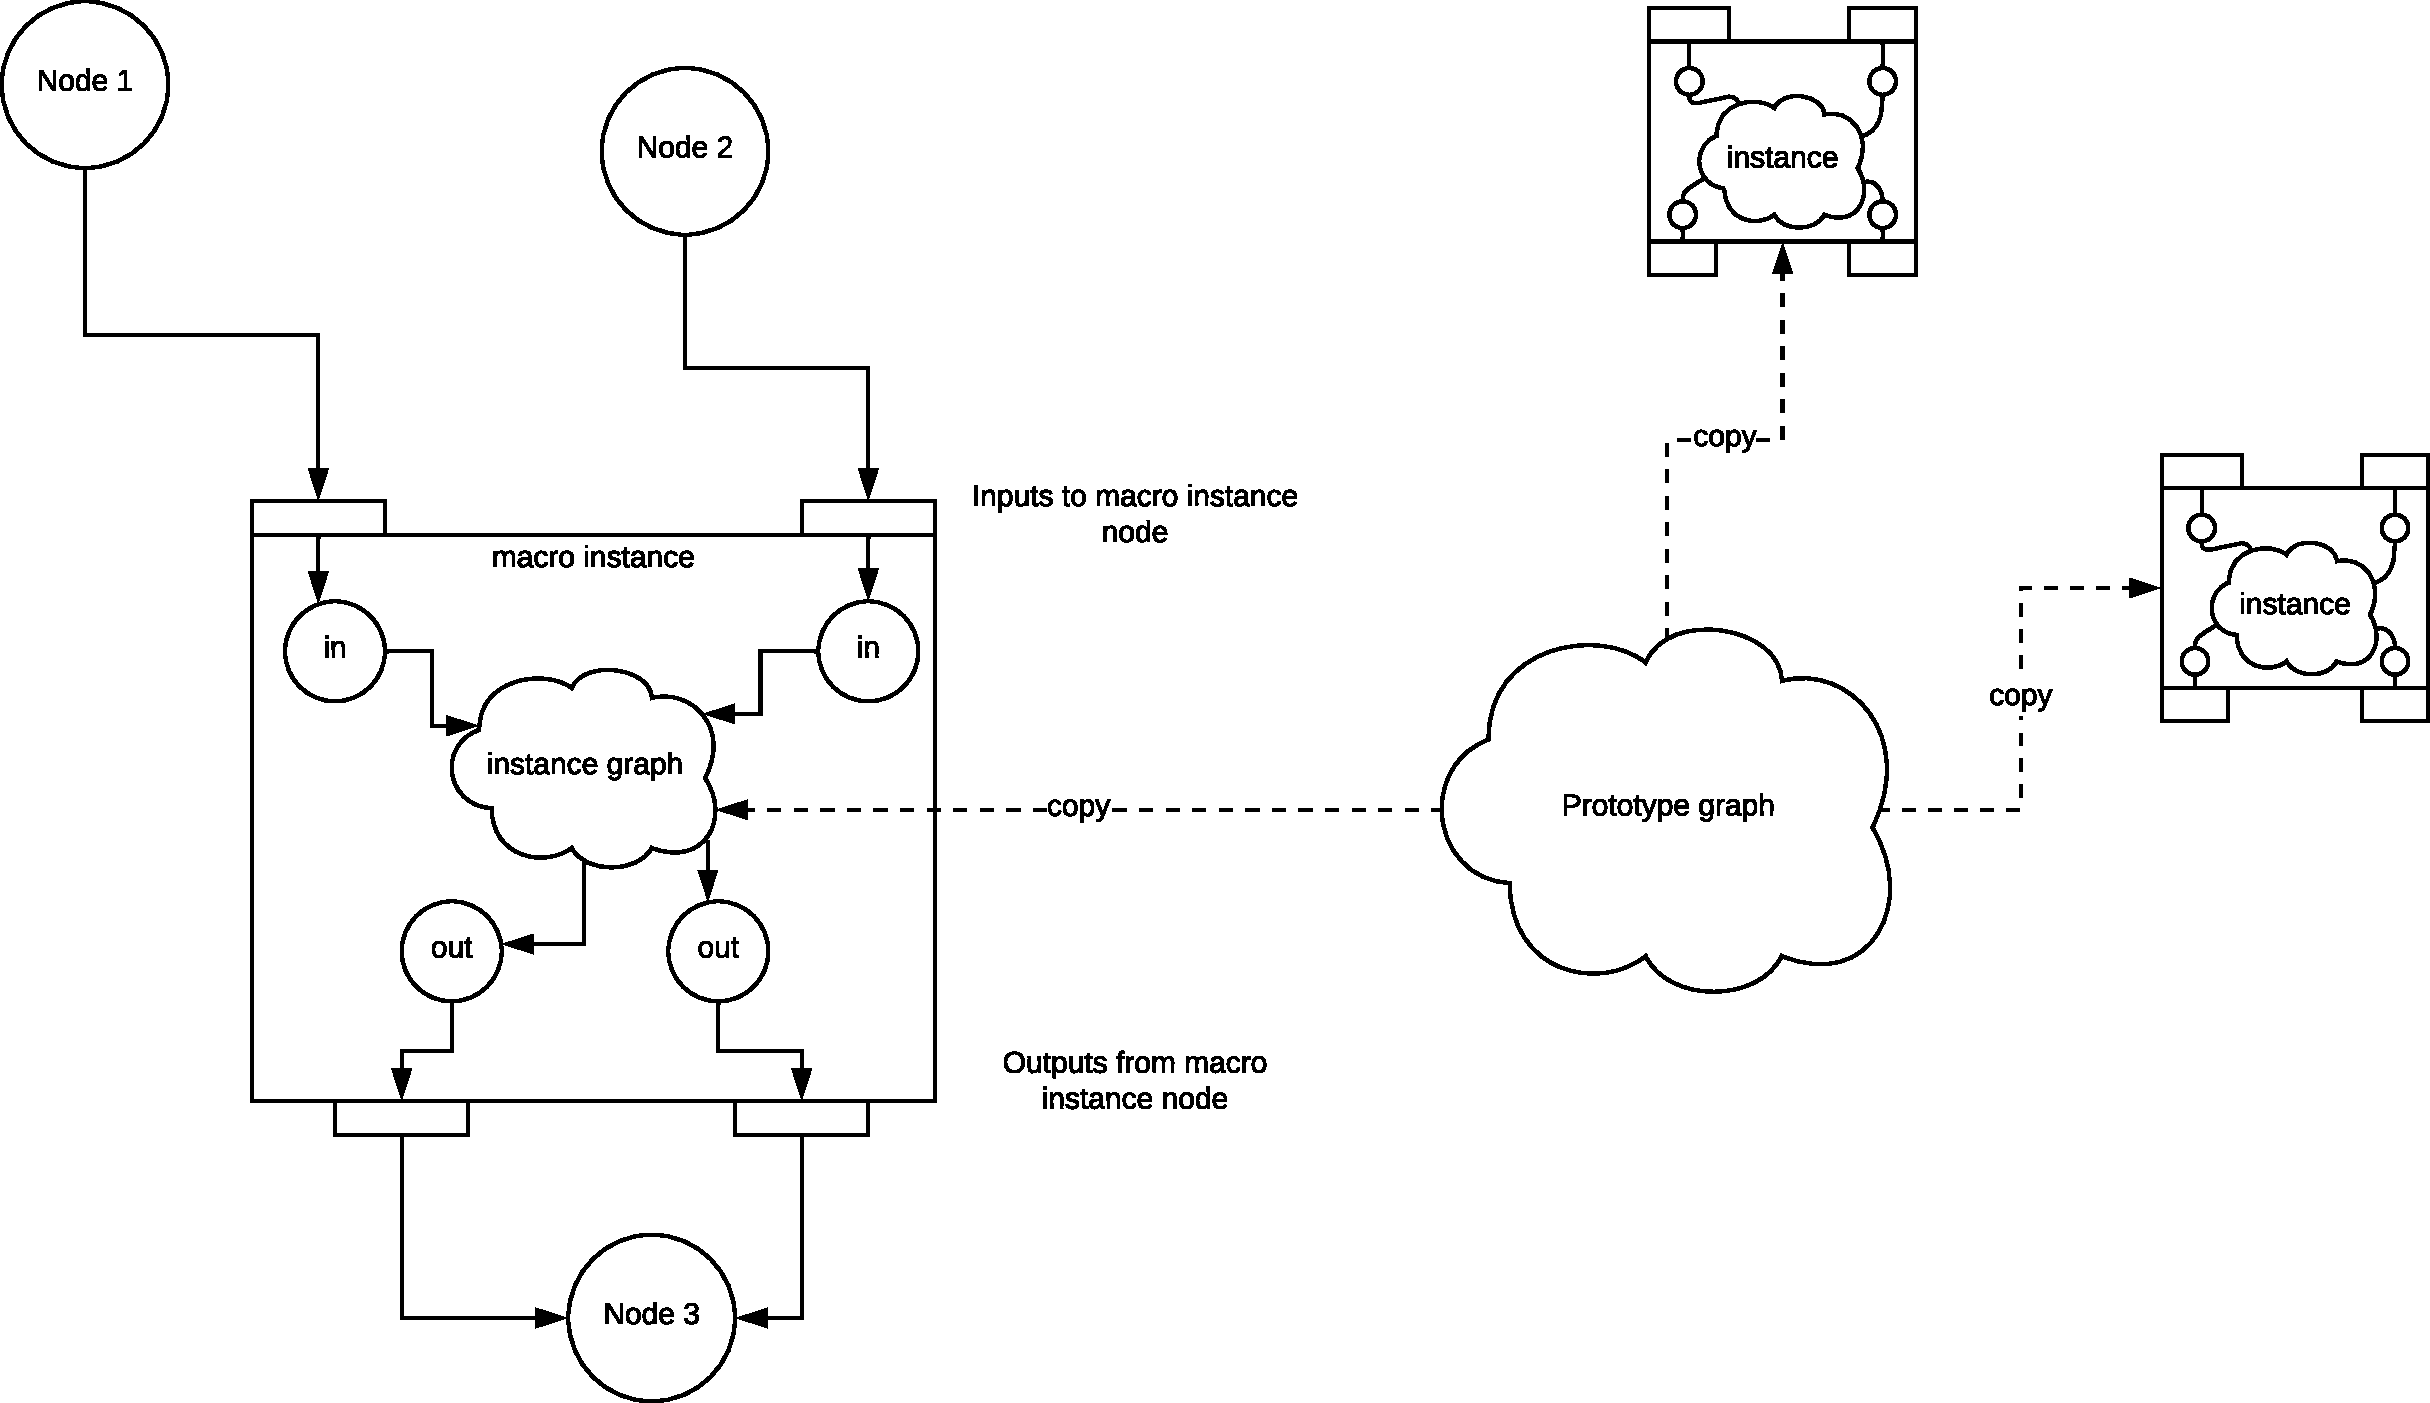
\includegraphics[width=5in]{macroobjs.pdf}
\caption{An example of a graph containing macros}
\label{macroobjs.pdf}
\end{figure}
This contains three instance nodes of a single macro. 
I have ``zoomed in'' on one of the instances, showing that it is connected
to three other nodes: two on its inputs, one on its outputs.
When this main graph runs, the following happens:
\begin{itemize}
\item Node 1 is able to run, does so, and sets its output
\item The macro instance cannot yet run
\item Node 2 is able to run, does so, and sets its output
\item The macro instance can now run:
\begin{itemize}
\item The macro instance node copies its input data
into the input nodes contained within the instance graph
\item The input nodes in the instance graph are run
\item The nodes dependent on those input nodes are run (i.e.\ the
instance graph proper)
\item The output nodes in the instance graph are run, copying their
inputs into the macro instance node's outputs
\item the instance now has now completed its run
\end{itemize}
\item Node 3 can now run, reading its inputs from the macro instance node.
\end{itemize}

\subsubsection{Macro inefficiencies}
\label{macroineff}
As noted above in Sec.~\ref{graphperform}, all the nodes in all instance
graphs are run whenever the prototype graph is changed. This is very
inefficient and may cause considerable delays. It's done by simply forcing all
\texttt{XFormMacro} nodes which are instances of the macro to perform themselves. Here
is the relevant part of \texttt{XFormGraph.changed()}:
\begin{lstlisting}
    # distribute changes in macro prototype to instances.
    # what we do here is go through all instances of the macro. 
    # We copy the changed prototype to the instances, then run
    # the instances in the graphs which contain them (usually the
    # main graph).
    # This could be optimised to run only the relevant (changed) component
    # within the macro, but that's very hairy.

    for inst in self.proto.instances:
        inst.instance.copyProto()
        inst.graph.performNodes(inst)
\end{lstlisting}
Here, \texttt{inst} is each \texttt{XFormMacro} node inside the main graph. Thus
\texttt{inst.graph} will be the main graph (for an non-nested macro). The
\texttt{self} value is the macro prototype graph, because this
method was called on an object inside that graph. This code therefore calls
\texttt{performNodes()} on the main graph to run the \texttt{XFormMacro} node inside
that graph. 

In an ideal world, this process --- calling \texttt{changed()} --- would identify
the instance node which corresponds to the prototype node which was changed, and only
run that inside the instance graph for the macro. The child nodes of the instance node
would then need to be run.


\subsection{User interface}
The user interface is mainly in the \texttt{ui} package, although each
node type's file contains its UI code (a subclass of \texttt{ui.tabs.Tab}.
A reasonably full view of the system is shown as a class diagram
in Fig.~\ref{ui.pdf}.
The main files involved are:
\begin{itemize}
\item \texttt{ui/mainwindow.py}: the main window classes;
\item \texttt{ui/tabs.py}: the \texttt{DocktableTabWindow} and \texttt{Tab}
classes (also the \texttt{ExpandedTab} class for when a tab is undocked);
\item \texttt{ui/canvas.py}: the Canvas widget for viewing image cube slices;
\item \texttt{ui/graphview.py}: contains \texttt{GraphView}, the
\texttt{QGraphicsView} subclass which encapulates a view on the graph scene;
\item \texttt{ui/graphscene.py}: contains \texttt{XFormGraphScene},
the \texttt{QGraphicsScene} subclass which contains a set of 2D objects
representing an \texttt{XFormGraph} and its nodes. It also contains the
classes representing those 2D objects (subclasses of various Qt graphics item
classes).
\end{itemize}
The input system's UI is not discussed here --- it's a separate
system in \texttt{ui/inputs.py}. See Sec.~\ref{inputs} for more details.


\begin{figure}[ht]
\center
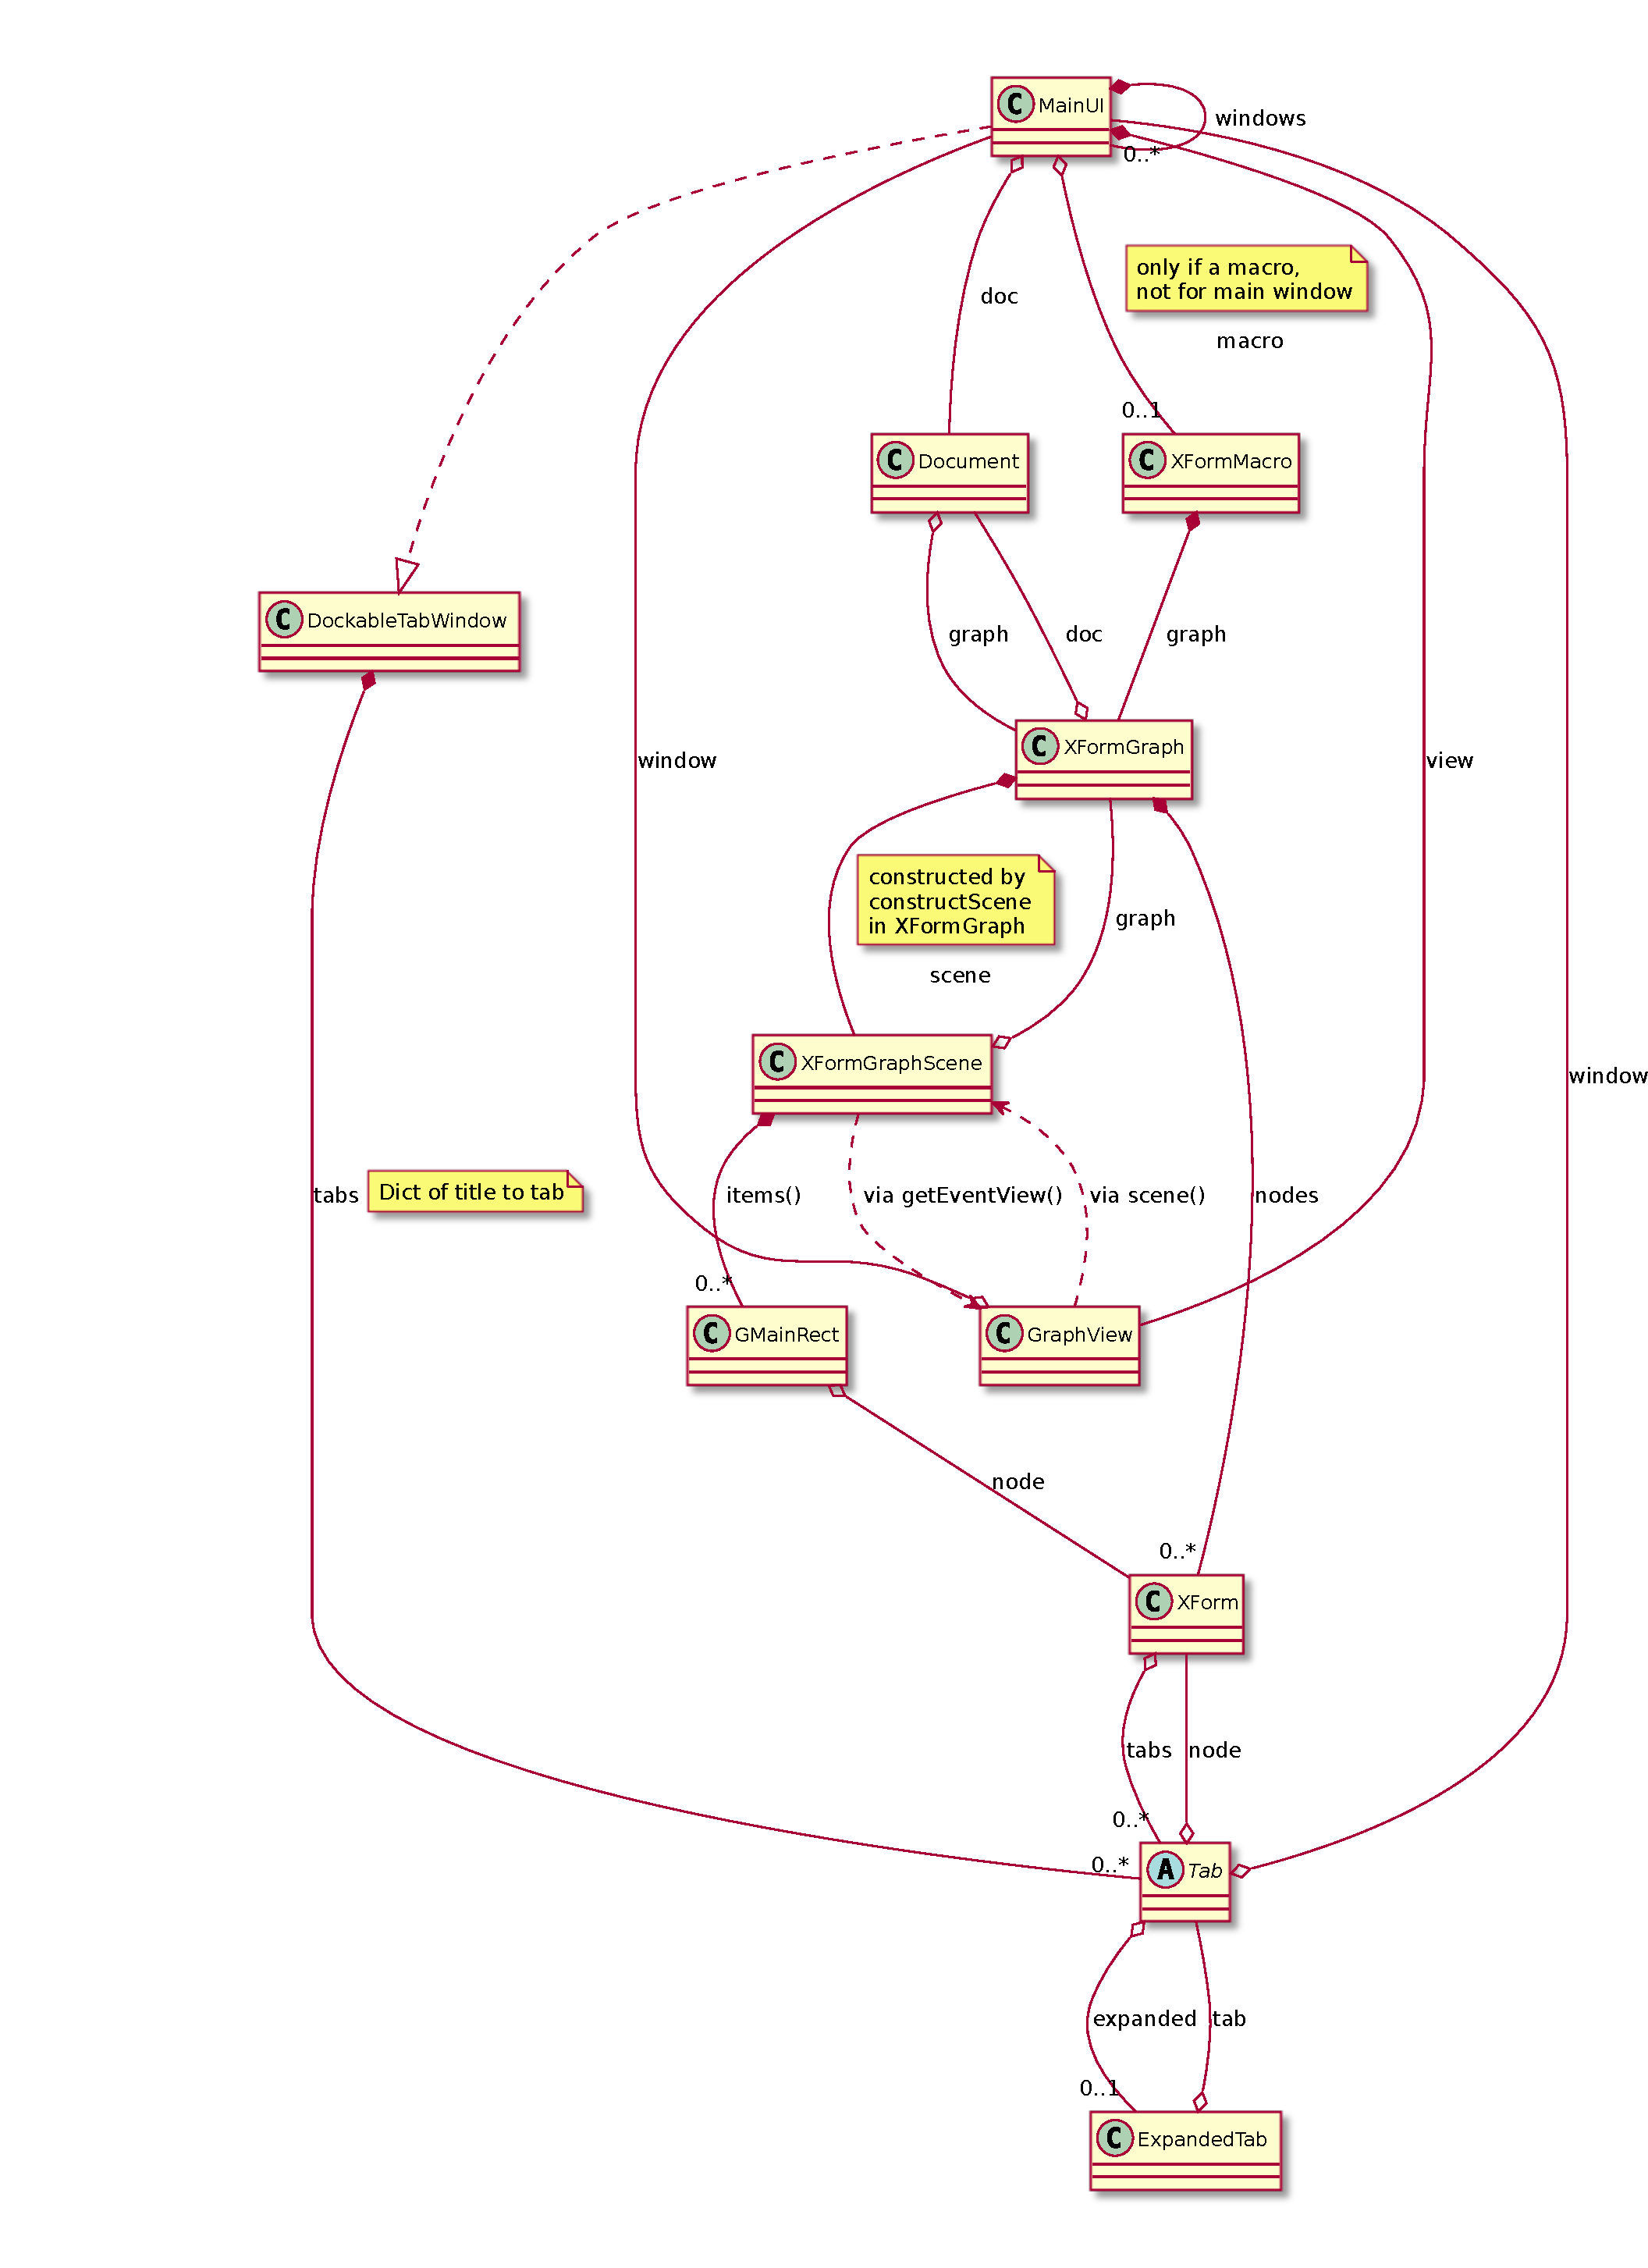
\includegraphics[width=4in]{ui.pdf}
\caption{UI class diagram}
\label{ui.pdf}
\end{figure}


\clearpage
\subsubsection{The main window}
The main window class is \texttt{ui.mainwindow.MainUI}. They contain the
following main widgets:
\begin{itemize}
\item a \texttt{QTabWidget} to hold the dockable tabs (tab docking is
handled by the \texttt{DocktableTab} superclass);
\item a \texttt{GraphView} widget to manage viewing and manipulating
the graph;
\item a \texttt{Palette} to contain the buttons to create new nodes
\end{itemize}
The bottom pane contains various widgets, such as the log console and
caption control combo box.
Main windows are created:
\begin{itemize}
\item when the application opens the first empty main graph in \texttt{main.py}
\item when a new, empty main graph window is created
\item when a window for a macro prototype graph is created
via \texttt{createMacroWindow()}.
\end{itemize}
There are some ownership oddities here. In the first two cases
the \texttt{MainUI} constructor is called with no arguments. This will
cause it to create a new \texttt{XFormGraph} which the window will own.
In the last case, the constructor is informed that the graph is a macro
prototype. This causes the UI to be created slightly differently. 
The \texttt{createMacroWindow()} static method then sets the graph to the macro's
prototype, which is owned by the \texttt{XFormMacro}.

In both cases, the \texttt{XFormGraphScene} contains a Qt Graphics Scene
which is constructed and regularly updated from the graph (by calling
its \texttt{rebuild()} method). This is viewed in
the main window through the \texttt{GraphView} class. Both these classes
accept various user actions and use them to modify the graph.

